% ═══════════════════════════════════════════════════════════
%  封面（三栏跨页：封底 21cm │ 书脊 3cm │ 封面 21cm）
%  —— 独立编译，产出 Cover.pdf
%
%  为什么与内文分开：
%    封面页宽 45cm，内文页宽 21cm。若合在一个 PDF，阅读器按最宽页
%    缩放/居中，会让 21cm 的正文页看起来挤在一侧（“内容往左偏”）。
%    分开后：内文全 21cm 统一；封面单独交印厂（印刷本就分开）。
%
%  编译：xelatex Cover.tex      （或 make cover）
% ═══════════════════════════════════════════════════════════
\documentclass[12pt]{book}
\usepackage{fontspec}
\usepackage{xcolor}
\usepackage{tikz}
\usepackage{graphicx}
% geometry 须与 TopologyBook.sty 一致：cover2 的版心补偿(\backoffset)依赖它
\usepackage[paperwidth=21cm, paperheight=29.7cm, left=1cm, right=1cm,
            top=1.2cm, bottom=1.5cm, includehead]{geometry}
\setmainfont{Times New Roman}

\begin{document}
% ═══════════════════════════════════════════════════════════
%  封面 / 书脊 / 封底（合版单页）
%  页面布局（左→右）：后封 21cm │ 书脊 3cm │ 前封 21cm
%    后封 = 封底：标题块 + 介绍文 + 出版社信息 + ISBN 条码
%    前封 = 封面：标题块 + 图案 + 作者
%  标题块由 \coverTitleBlock 统一提供（前后封共用，改一处即两处同步）
% ═══════════════════════════════════════════════════════════

% ── 颜色 ──
\definecolor{covercolor}{HTML}{315758}
\definecolor{linecolor}{HTML}{D6E19A}

% ── 尺寸参数 ──
\newlength{\spinewidth}
\setlength{\spinewidth}{3cm}                 % 书脊宽
\newlength{\patternwidth}
\setlength{\patternwidth}{14.4cm}            % 图案/副标题基准宽

% 封底版心：左右内缩 \backinset（同值 → 左右对称）
\newlength{\backinset}
\setlength{\backinset}{1.8cm}
% 文字块(\textwidth)左缘相对【面板左缘】的偏移。
% 说明：\textwidth ≠ 面板宽(21cm)，且文字块自页边距起排，故内容需按此补偿才能对齐面板。
%       值为 LaTeX 标准的文字块左边距 = 1in + \hoffset + \oddsidemargin。
\newlength{\backoffset}
\setlength{\backoffset}{\dimexpr 1in+\hoffset+\oddsidemargin\relax}
% 封底版心宽 = 面板宽 − 左右内缩（各含 \backoffset 补偿）
\newlength{\backcontentwidth}
\setlength{\backcontentwidth}{\dimexpr 21cm-2\backinset-2\backoffset\relax}

% ── 字体 ──
\newfontfamily{\SenatorTall}{SenatorTall.otf}
\newfontfamily{\RebarBold}{rebar-bold-1.ttf}
\newfontfamily{\Trajan}{TrajanPro-Regular.otf}

% ── 图案（黑白几何花形，仅封面用）──
\newcommand{\reversedpattern}{%
    \begin{tikzpicture}[x=0.5\patternwidth/6, y=0.5\patternwidth/6,
        armfill/.style={fill=covercolor,draw=linecolor,line width=2.2pt},
        armline/.style={draw=linecolor,line width=2.2pt},
        arm/.pic={
            \draw[##1]
                (0,0) |- (4,4)
                -- ++(0,-\fpeval{4*(2-sqrt(2))})
                -- (45:4) -- cycle;
        }
    ]
        % 底层：光晕
        \draw[line width=3pt,linecolor,fill=covercolor] (-6,-6) rectangle (6,6);
        \foreach \i in {5.8, 5.75, ..., 3.9} {
            \def\tmp{\fpeval{100*(\i/5.8)}}
            \fill[covercolor!\tmp!white] circle[radius=\i];
        }
        % 8臂填充
        \foreach \angle in {0,45,...,315} { \pic[rotate=\angle] {arm={armfill}}; }
        % 顶层：指数衰减高光
        \begin{scope}
            \clip (-6,-6) rectangle (6,6);
            \foreach \i in {0,1,...,100} {
                \pgfmathsetmacro{\radius}{\i/50*5.0}
                \pgfmathsetmacro{\opacity}{0.15 * exp(-\radius/1.2)}
                \fill[white, opacity=\opacity] (0,0) circle (\radius);
            }
        \end{scope}
        % 8臂边框
        \foreach \angle in {0,45,...,315} { \pic[rotate=\angle] {arm={armline}}; }
    \end{tikzpicture}%
}

% ── 标题块（前封/后封共用）──
% 依赖调用处的 \centering 环境；两侧用同一宏 → 位置/字体完全一致
\newcommand{\coverTitleBlock}{%
    \color{white}%
    \vspace*{0.2cm}%
    % TOPOLOGY（逐字拉伸铺满 \textwidth）
    {\centering
    \SenatorTall
    \fontsize{60}{0}\selectfont
    \noindent\makebox[\textwidth][s]{%
    \raisebox{1em}{\scalebox{3}[2.9]{T}}\hfill%
    \raisebox{1em}{\scalebox{3}[2.9]{O}}\hfill%
    \raisebox{1em}{\scalebox{3}[2.9]{P}}\hfill%
    \raisebox{1em}{\scalebox{3}[2.9]{O}}\hfill%
    \raisebox{1em}{\scalebox{3}[2.9]{L}}\hfill%
    \raisebox{1em}{\scalebox{3}[2.9]{O}}\hfill%
    \raisebox{1em}{\scalebox{3}[2.9]{G}}\hfill%
    \raisebox{1em}{\scalebox{3}[2.9]{Y}}%
    }
    \par}%
    \vspace{-1cm}%
    % SECOND EDITION
    \noindent
    \begin{minipage}{\patternwidth}
        \centering
        \RebarBold
        \color{linecolor}\fontsize{20}{0}\selectfont
        S\hspace{0.95em}E\hspace{0.95em}C\hspace{0.95em}O\hspace{0.95em}N\hspace{0.95em}D%
        \hfill%
        E\hspace{0.95em}D\hspace{0.95em}I\hspace{0.95em}T\hspace{0.95em}I\hspace{0.95em}O\hspace{0.95em}N%
    \end{minipage}%
}

% ═══════════════════════════════════════════════════════════
%  页面：扩展为 2×页宽 + 书脊（三栏合版）
% ═══════════════════════════════════════════════════════════
\pagecolor{covercolor}
\thispagestyle{empty}

\cleardoublepage
\thispagestyle{empty}

\newdimen\savepagewidth
\savepagewidth=\pdfpagewidth
\pdfpagewidth=\dimexpr 2\savepagewidth + \spinewidth\relax

% 前封距面板左缘的偏移 = 后封 + 书脊
\newdimen\frontshift
\frontshift=\dimexpr \savepagewidth + \spinewidth\relax

% ── 书脊（TikZ overlay：分界线 + 竖排文字）──
\begin{tikzpicture}[remember picture,overlay]
    \draw[linecolor,line width=0.8pt]     % 后封/脊
        ([xshift=\savepagewidth]current page.north west) --
        ([xshift=\savepagewidth]current page.south west);
    \draw[linecolor,line width=0.8pt]     % 脊/前封
        ([xshift=\frontshift]current page.north west) --
        ([xshift=\frontshift]current page.south west);
    \node[rotate=-90, anchor=center, text=linecolor,
          font=\RebarBold\fontsize{26}{30}\selectfont]
        at ([xshift=\dimexpr\savepagewidth+0.5\spinewidth\relax]current page.west)
        {ZY6412 \hspace{1.2em} Topology \hspace{1.2em} 2nd};
\end{tikzpicture}

% ═══════════════════════════════════════════════════════════
%  前封 / 后封 内容盒
%  两盒各装进 \sbox 量高，再用 \raisebox 抬起后封 → 顶部对齐
%  （默认 [c] 为基线对齐，两盒等高才顶齐；此处用抬升量补偿高度差）
% ═══════════════════════════════════════════════════════════

% ── 前封：标题块 + 图案 + 作者 ──
\newsavebox{\coverfrontbox}
\sbox{\coverfrontbox}{%
    \begin{minipage}{\textwidth}
    \begingroup
        \centering
        \coverTitleBlock
        \vspace{1.7cm}

        \reversedpattern

        \vspace{2em}
        \vfill

        % 作者
        {\centering
        \Trajan
        \color{linecolor}\fontsize{38}{0}\selectfont
        \makebox[\patternwidth][s]{JAMES\hspace{0.3em} R.\hspace{0.3em} MUNKRES}
        \par}
        \vspace{0.1cm}
    \endgroup
    \end{minipage}%
}

% ── 后封：标题块 + 介绍文 + （出版社 | ISBN 条码）──
% 高度固定为 文字块高 − 下边距，使底部内容贴近版心底
\newsavebox{\coverbackbox}
\sbox{\coverbackbox}{%
    \begin{minipage}[t][\dimexpr\textheight-2.5cm\relax]{\textwidth}
    \begingroup
        \centering
        \coverTitleBlock
        \par
    \endgroup

    % 介绍文字（书名 Topology 斜体；版心与下方一致 → 左缘对齐）
    \vspace{2.5cm}
    \begingroup
        \color{white}
        \noindent\hspace*{\backinset}%
        \begin{minipage}{\backcontentwidth}
            \fontsize{13}{20}\selectfont
            \noindent\textit{Topology}, 2nd edition is designed to provide instructors with a convenient single text resource for bridging general and algebraic topology courses. 2 separate, distinct sections (1 on general point-set topology, the other on algebraic topology) are each suitable for a one-semester course and are based around the same set of basic core topics. Optional, independent topics and applications can be studied and developed in depth depending on course needs and preferences. This title is part of the Pearson Modern Classics series. Pearson Modern Classics are acclaimed titles at a value price.\par
        \end{minipage}
    \endgroup

    \vfill

    % 版心底：出版社信息（左） + ISBN 条码（右）
    \begingroup
        \color{white}
        \noindent\hspace*{\backinset}%
        \begin{minipage}[b]{\backcontentwidth}%
            \noindent
            % 左：出版社（Trajan 名号 + Times 地址/网址，网址须保持小写）
            \begin{minipage}[b]{9cm}
                \raggedright
                {\Trajan\fontsize{14}{17}\selectfont PRENTICE HALL\par}
                \vspace{0.6em}
                {\rmfamily\fontsize{10}{13}\selectfont
                 Upper Saddle River, NJ 07458\par}
                \vspace{0.2em}
                {\rmfamily\fontsize{10}{13}\selectfont
                 http://www.prenhall.com\par}
            \end{minipage}%
            \hfill
            % 右：ISBN 条码（矢量 PDF；白底以保证可扫描）
            \begin{minipage}[b]{5.5cm}
                \raggedleft
                \colorbox{white}{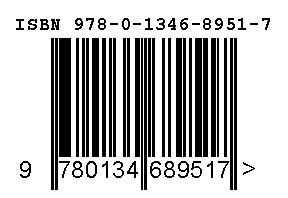
\includegraphics[width=4.32cm]{images/isbn_barcode.pdf}}
            \end{minipage}%
        \end{minipage}%
    \endgroup
    \end{minipage}%
}

% ── 叠放：后封在左（抬起顶对齐，\smash 免撑行高）；前封在右（\frontshift 偏移）──
\noindent
\rlap{\smash{\raisebox{\dimexpr\ht\coverfrontbox-\ht\coverbackbox\relax}{\usebox{\coverbackbox}}}}%
\rlap{\hspace{\frontshift}\usebox{\coverfrontbox}}

\clearpage
\pdfpagewidth=\savepagewidth
\nopagecolor

\end{document}
